\section{What is optimisation?}

Optimisation is one of these words that has many meanings, depending on the context you take as a reference. In the context of this book, optimisation refers to \emph{mathematical optimisation}, which is a discipline of applied mathematics.

In mathematical optimisation, we build upon concepts and techniques from calculus, analysis, linear algebra, and other domains of mathematics to develop methods to find values for variables (or solutions) within a given domain that maximise (or minimise) the value of a function. In specific, we are trying to solve the following general problem:
%
\begin{align}
    \mini & f(x) \label{p1c1:eq:opt_prob} \\
    \st   & x \in X. \nonumber
\end{align}
%
That is, we would like to find the solution $x$ that \emph{minimises} the value of the \emph{objective function} $f$, such that (s.t.) $x$ belongs to the \emph{feasibility set} $X$. In a general sense, problems like this can be solved by employing the following strategy:
%
\begin{enumerate}
    \item Analysing properties of the function $f(x)$ under specific domains and deriving the conditions that must be satisfied such that a point $x$ is a candidate optimal point.
    \item Applying numerical methods that iteratively search for points satisfying these conditions. 
\end{enumerate}
%
This idea is central in several knowledge domains and often is described with area-specific nomenclature. Fields such as economics, engineering, statistics, machine learning and, perhaps more broadly, operations research, are intensive users and developers of optimisation theory and applications. 

\subsection{Mathematical programming and optimisation}

Operations research and mathematical optimisation are somewhat intertwined, as they both were born around a similar circumstance. %(Include something on the history of OR)

I personally like to separate \emph{mathematical programming} from (mathematical) \emph{optimisation}. Mathematical programming is a modelling paradigm in which we rely on (very powerful, I might add) analogies to model \emph{real-world} problems. In that, we look at a given decision problem considering that:
%
\begin{itemize}
    \item \emph{variables} represent \emph{decisions}, as in a business decision or a course of action. Examples include setting the parameters of (e.g., prediction) models, production systems layouts, geometries of structures, topologies of networks, and so forth; 
    \item \emph{domain} represents business rules or \emph{constraints}, representing logic relations, design or engineering limitations, requirements, and such; 
    \item \emph{objective function} is a function that provides a measure of solution quality.  
\end{itemize}
%    
With these in mind, we can represent the decision problem as a \emph{mathematical programming model} of the form of \eqref{p1c1:eq:opt_prob} that can be solved using \emph{optimisation} methods. From now on, we will refer to this specific class of models as mathematical optimisation models, or optimisation models for short. We will also use the term \emph{solve the problem} to refer to the task of finding optimal solutions to optimisation models.

This book mostly focuses on the optimisation techniques employed to find optimal solutions for these models. As we will see, depending on the nature of the functions that are used to formulate the model, some methods might be more or less appropriate. Further complicating the issue, for models of a given nature, there might be alternative algorithms that can be employed and with no generalised consensus on whether one method is generally better performing than another, which is one of the aspects that make optimisation so exciting and multifaceted when it comes to alternative approaches. I hope that this makes more sense as we progress through the chapters. 


\subsection{Types of mathematical optimisation models}

In general, the simpler the assumptions on the parts forming the optimisation model, the more efficient the methods to solve such problems. 

Let us define some additional notation that we will use from now on. Consider a model in the general form
%
\begin{align*}
	\mini & f(x) \\
	\st   & g_i(x) \leq 0, ~i = 1, \dots, m \\
	      & h_i(x) = 0, ~i = 1, \dots, l \\
	      & x \in X,  
\end{align*}
%
where $f: \reals^n \mapsto \reals$ is the objective function, $g:\reals^n \mapsto \reals^m$ is a collection of $m$ inequality constraints and $h: \reals^n \mapsto \reals^l$ is a collection of $l$ equality constraints.

In fact, every inequality constraint can be represented by an equality constraint by making $h_i(x) = g_i(x) + x_{n+1}$ and augmenting the decision variable vector $x \in \reals^n$ to include the slack variable $x_{n+1}$. However, since these constraints behave very differently from an algorithmic standpoint, we will explicitly represent both whenever necessary.

The most general types of models are the following. We also use this as an opportunity to define some (admittedly confusing) nomenclature from the field of operations research that we will be using in these notes.
%
\begin{enumerate}
    \item \emph{Unconstrained models:} in these, the set $X = \reals^n$ and $m=l=0$. These are prominent in, e.g., machine learning and statistics applications, where $f$ represents a measure of model fitness or prediction error.  
    \item \emph{Linear programming (LP):} presumes linear objective function $f(x) = c^\top x$ and affine constraints $g$ and $h$, i.e., of the form $a_i^\top x - b_i$, with $a_i \in \reals^n$ and $b \in \reals$. Normally, $X = \braces{x \in \reals^n \mid x_j \geq 0, j = 1,\dots, n}$ enforce that the domain of the decision variables is the nonnegative orthant.
    \item \emph{Nonlinear programming (NLP):} some or all of the functions $f$, $g$, and $h$ are nonlinear.
    \item \emph{Mixed-integer (linear) programming (MIP):} consists of an LP in which some (or all, being then simply integer programming) of the variables are constrained to be integers. In other words, $X \subseteq \reals^k \times \integers^{n-k}$. Very frequently, the integer variables are constrained to be binary terms, i.e., $x_i \in \braces {0,1}$, for $i = 1,\dots, n-k$ and are meant to represent true-or-false or yes-or-no conditions.
    \item \emph{Mixed-integer nonlinear programming (MINLP):} are the intersection of MIPs and NLPs.  
\end{enumerate}

{\bf Remark:} notice that we use the vector notation $c^\top x = \sum_{j \in J} c_j x_j$, with $J = \braces{1,\dots,N}$. This is just a convenience for keeping the notation compact. 


\section{Linear programming applications}

We will consider now a few examples of liner programming models with somewhat general structure. Many of these examples have features that can be combined into more general models.


\subsection{Resource allocation} \label{section_121}

Most linear programming (LP) problems can be interpreted as a \emph{resource allocation} problem. In that, we are interested in defining an optimal allocation of resources (i.e., a plan) that maximises return or minimises costs and satisfies allocation rules. 

Specifically, let $I = \braces{1, \dots, i, \dots, m}$ be a set of resources that can be combined to produce products in the set $J = \braces{1, \dots, j, \dots, n}$. Assume that we are given a return $c_j$ per unit of product $j$, $\forall j \in J$, and a list of $a_{ij}$, $\forall i \in I, \forall j \in J$, describing which and how much of the resources $i \in I$ are required for making product $j \in J$. Assume that the availability $b_i$ of resource $i$, $\forall i\in I$, is known. 

Our objective is to define the amounts $x_j$ representing the production of $j \in J$. We would like to define those in a way that we optimise the resource allocation plan quality (in our case, maximise return from the production quantities $x_j$) while making sure the resources needed for production do not exceed the availability of resources. For that, we need to define: 

The \emph{objective function}, which measures the \emph{quality} of a production plan. In this case, the total return for a given plan is given by:
%
\begin{equation*}
	\maxi \sum_{j \in J}c_jx_j \Rightarrow c^\top x,
\end{equation*}
%
where $c = [c_1, \dots, c_{N}]^\top$ and $x = [x_1, \dots, x_{N}]^\top$ are $n$-sized vectors. Notice that $c^\top x$ denotes the inner (or dot) product. The transpose sign $^\top$ is meant to reinforce that we see our vectors as column vectors, unless otherwise stated.

Next, we need to define \emph{constraints} that state the conditions for a plan to be \emph{valid}. In this context, a valid plan is a plan that does not utilise more than the amount of available resources $b_i$, $\forall i \in I$. This can be expressed as the collection (one for each $i \in I$) of affine (more often wrongly called, as we will too, linear) inequalities
%
\begin{equation*}
	\st \sum_{j \in J} a_{ij}x_j \leq b_i, \forall i \in I	\Rightarrow	Ax \leq b,
\end{equation*}
%
where $a_{ij}$ are the components of the $M \times N$ matrix $A$ and $b = [b_1,\dots, b_M]^\top$. Furthermore, we also must require that $x_i \geq 0, \forall i \in I$.                                                                                                         

Combining the above, we obtain the generic formulation that will be used throughout this text to represent linear programming models:
%
\begin{align}
	\maxi & c^\top x  \label{p1c1:eq:LP_objective} \\
	\st   & Ax \leq b \label{p1c1:eq:LP_constraint} \\
		  & x \geq 0. \label{p1c1:eq:LP_domain}
\end{align}
%


\subsubsection{Illustrative example: the paint factory problem} \cite{taha2003operations}
 
Let us work on a more specific example that will be useful for illustrating some important concepts related to the geometry of linear programming problems.

Let us consider a paint factory that produces \emph{exterior} and \emph{interior paint} from raw materials \emph{M1} and \emph{M2}. The \emph{maximum demand} for interior paint is 2 tons/day. Moreover, the amount of interior paint produced \emph{cannot exceed} that of exterior paint by more than 1 ton/day. 

Our goal is to determine the optimal paint production plan. Table \ref{p1c1:tab:paint_factory_problem_data} summarises the data to be considered. Notice the constraints that must be imposed to represent the daily availability of paint.

\begin{table}[h]
	\begin{tabular}{rccc} \hline
	&\multicolumn{2}{c}{material (ton)/paint (ton)}\\ \hline
	& exterior paint & interior paint & daily availability (ton)\\ \hline
	material M1 & 6 & 4 & 24\\
	material M2 & 1 & 2 & 6\\ \hline
	profit (\$1000 /ton) & 5 & 4\\ \hline
	\end{tabular}
	\caption{Paint factory problem data} \label{p1c1:tab:paint_factory_problem_data}
\end{table}

The paint factory problem is an example of a resource allocation problem. Perhaps one aspect that is somewhat dissimilar is the constraint representing the production rules regarding the relative amounts of exterior and interior paint. Notice, however, that this type of constraint also has the same format as the more straightforward resource allocation constraints.  

Let $x_1$ be the amount produced of exterior paints (in tons) and $x_2$ the amount of interior paints. The complete model that optimises the daily production plan of the paint factory is:
%
\begin{flalign}
	\maxi z = \ & 5x_1 + 4x_2 \label{p1c1:eq:constM1}\\
	\st & 6x_1 + 4x_2 \leq 24 \label{p1c1:eq:constM2}\\
	& x_1 + 2x_2 \leq 6 \\
	& x_2 - x_1 \leq  1 \\
	& x_2 \leq 2 \\
	& x_1, x_2 \geq 0
\end{flalign}
%
Notice that paint factory model can also be \emph{compactly represented} as in \eqref{p1c1:eq:LP_objective}--\eqref{p1c1:eq:LP_domain}, where
%
\begin{equation*}
	c = [5, 4]^\top, \ x = [x_1, x_2]^\top, \ A = \begin{bmatrix} 6 & 4 \\ 1 & 2 \\ -1 & 1 \\0 & 1 \end{bmatrix}, \text{ and } b = [24, 6, 1, 2]^\top.	
\end{equation*}
%


\subsection{Transportation problem}

Another important class of linear programming problems is those known as transportation problems. These problems are often modelled using the abstraction of graphs since they consider a network of nodes and arcs through which some flow must be optimised. Transportation problems have several important characteristics that can be exploited to design specialised algorithms, the so-called \emph{transportation simplex} method. Although we will not discuss these methods in this text, the simplex method (and its variant, the dual simplex method) will be at the centre of our developments later on. Also, modern solvers have increasingly relegated transport simplex methods in their development, as dual simplex has consistently shown to perform similarly in the context of transportation problems, despite being a far more general method. 

The problem can be summarised as follows. We would like to plan the production and distribution of a certain product, taking into account that the transportation cost is known (e.g., proportional to the distance travelled), the factories (or source nodes) have a capacity limit, and the clients (or demand nodes) have known demands. Figure \ref{p1c1:fig1:transport_network} illustrates a small network with two factories, located in San Diego and Seattle, and three demand points, located in New York, Chicago, and Miami. Table \ref{p1c1:tab:transport_problem_data} presents the data related to the problem. 
%
\begin{figure}[h]
	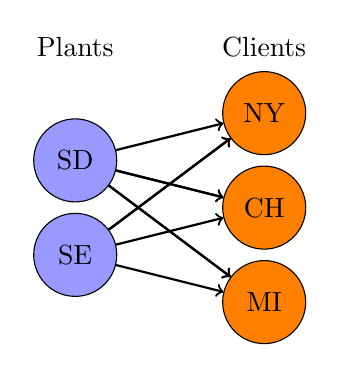
\begin{tikzpicture}[scale=1.2,
		node/.style={circle, fill=blue!40, draw, minimum size=3em, inner sep=1pt},
		node2/.style={circle, fill=orange, draw, minimum size=3em, inner sep=1pt}] 
    	\node[above] at (0, 3.5) {Plants};                                                                                  
    	\node[above] at (2, 3.5) {Clients};
	    \node[node] (1) at (0, 1.5) {SE};
	    \node[node] (2) at (0, 2.5) {SD};
	    \node[node2] (3) at (2, 3) {NY};
	    \node[node2] (4) at (2, 2) {CH};
	    \node[node2] (5) at (2, 1) {MI};
	    \foreach \x in {1,...,2} {
	       \foreach \y in {3,...,5} {
	          \draw[->, thick] (\x) -- (\y);
	          }}      
	    \draw[->, thick] (1) -- (3);
	    \draw[->, thick] (2) -- (4);
	    \draw[->, thick] (2) -- (5);                            
	\end{tikzpicture}
	\caption{Schematic illustration of a network with two source nodes and three demand nodes} \label{p1c1:fig1:transport_network}    
\end{figure}
%
\begin{table}[h]
	\begin{tabular}{r|ccc|c}
    	& & {\it Clients} &\\\hline
    	{\it Factory} & NY & Chicago & Miami & Capacity \\\hline
    	Seattle & 2.5      & 1.7    & 1.8   & 350 \\
    	San Diego & 3.5 & 1.8 & 1.4 & 600 \\\hline
    	Demands & 325 & 300 & 275 & - \\\hline
	\end{tabular}
	\caption{Problem data: unit transportation costs, demands and capacities} \label{p1c1:tab:transport_problem_data}
\end{table}

To formulate a linear programming model representing the transportation problem, let $i \in I = \{\text{Seattle}, \text{San Diego}\}$ be the index set representing factories. Similarly, let $j \in J = \{\text{New York}, \lb \text{Chicago}, \text{Miami}\}$.

The decisions, in this case, are represented by $x_{ij}$, which represents the amount produced in factory $i$ and sent to client $j$. Such a distribution plan can then be assessed by its total transportation cost, which is given by
%
$$ 
\mini z = 2.5x_{11} + 1.7x_{12} + 1.8x_{13} + 3.5x_{21} + 1.9x_{22} + 1.4x_{23}.
$$
%
The total transportation cost can be more generally represented as
%
$$
\mini z = \sum_{i \in I}\sum_{j \in J}c_{ij}x_{ij}
$$
%
where $c_{ij}$ is the unit transportation cost from $i$ to $j$.
%
The problem has two types of constraints that must be observed, relating to the supply capacity and demand requirements. These can be stated as the following linear constraints
%
\begin{align*}
	& x_{11} + x_{12} + x_{13} \leq 350 \text{ (capacity limit in Seattle)}\\
	& x_{21} + x_{22} + x_{23} \leq 600 \text{ (capacity limit in San Diego)}\\
	& x_{11} + x_{21} \geq 325 \text{ (demand in New York)}\\
	& x_{12} + x_{22} \geq 300 \text{ (demand in Chicago)}\\
	& x_{13} + x_{23} \geq 275 \text{ (demand in Miami)}.
\end{align*}
%
These constraints can be expressed in the more compact form
%
\begin{align}
	& \sum_{j \in J} x_{ij} \leq C_i, ~\forall i \in I \label{p1c1:eq:transportation_constraint_supply}\\
	& \sum_{i \in I} x_{ij} \geq D_j, ~\forall j \in J, \label{p1c1:eq:transportation_constraint_demand}
\end{align}

where $C_i$ is the production capacity of factory $i$ and $D_j$ is the client demand $j$. Notice that the terms on the lefthand side in \eqref{p1c1:eq:transportation_constraint_supply} accounts for the total production in each of the source nodes $i \in I$. Analogously, in constraint \eqref{p1c1:eq:transportation_constraint_demand}, the term on the left accounts for the total of the demand satisfied at the demand nodes $j \in J$. 

Using an optimality argument, we can see that any solution for which, for any $j \in J$, $\sum_{i \in I} x_{ij} > D_j$ can be improved by making $\sum_{i \in I} x_{ij} = D_j$. This show that this constraint under these conditions will always be satisfied as an equality constraint instead and could be replaced like such. 

The complete transportation model for the example above can be stated as 
%
\begin{align*}
	\mini z = \ &2.5x_{11} + 1.7x_{12} + 1.8x_{13} + 3.5x_{21} + 1.9x_{22} + 1.4x_{23} \\
	\st & x_{11} + x_{12} + x_{13} \leq 350, \ 
	x_{21} + x_{22} + x_{23} \leq 600\\
	& x_{11} + x_{21} \geq 325, \ x_{12} + x_{22} \geq 300, \ x_{13} + x_{23} \geq 275\\
	& x_{11}, \dots, x_{23} \geq 0.
\end{align*}
%

Or, more compactly, in the so-called \emph{algebraic (or symbolic) form}
%
\begin{align*}
	\mini z = \ &\sum_{i \in I}\sum_{j \in J}c_{ij}x_{ij} \\
	\st & \sum_{j \in J} x_{ij} \leq C_i, ~\forall i \in I \\
	& \sum_{i \in I} x_{ij} \geq D_j, ~\forall j \in J \\
	&x_{ij} \geq 0, \forall i \in I, ~\forall j \in J.
\end{align*}
%
One interesting aspect to notice regarding algebraic forms is that they allow to represent the main structure of the model while being independent of the instance being considered. For example, regardless of whether the instance would have 5 or 50 nodes, the algebraic formulation is the same, allowing for detaching the problem instance (in our case the 5 node network) from the model itself. Moreover, most computational tools for mathematical programming modelling (hereinafter referred to simply as modelling - like JuMP) empowers the user to define the optimisation model using this algebraic representation.

Algebraic forms are the main form in which we will specify optimisation models. This abstraction is a peculiar aspect of mathematical programming and is perhaps one of its main features, the fact that one must \emph{formulate} models for each specific setting, which can be done in multiple ways and might have consequences for how well an algorithm performs computationally. Further in this text, we will discuss this point in more detail.  


\subsection{Production planning (lot-sizing)}

Production planning problems, commonly referred to as lot-sizing problems in contexts related to industrial engineering, consider settings where a planning horizon is taken into consideration. Differently from the previous examples, lot-sizing problems allow for the consideration of a time flow aspect, in which production that takes place in the past can be ``shifted'' to a future point in time by means of inventories (i.e., stocks). Inventories are important because they allow for taking advantage of different prices at different time periods, circumventing production capacity limitations, or preparing against uncertainties in the future (e.g., uncertain demands).

The planning horizon is represented by a collection of chronologically ordered elements $t \in \braces{1,\dots, T}$ representing a set of uniformly-sized time periods (e.g., months or days). Then, let us define the decision variables $p_t$ as the amount produced in period $t$ and $k_t$ the amount stored in period $t$, which is available for use in periods $t' > t$. These decisions are governed by two costs: $P_t$, $\forall t \in T$, representing the production cost in each time period $t$ and the unit holding cost $H$, that is, how much it costs to hold one unit of product for one time period. 

Our objective is to satisfy the demands $D_t$, $\forall t \in T$, at the minimum possible cost. Figure \ref{p1c1:fig:lot-sizing_diagram}	provides a schematic representation of the process to be modelled. Notice that each node represents a material balance to be considered, that is, that at any period $t$, the total produced plus the amount held in inventory from the previous period ($t-1$) must be the same as the amount used to satisfy the demand plus the amount held in inventory for the next period ($t+1$). 	
   
\begin{figure}[h]
	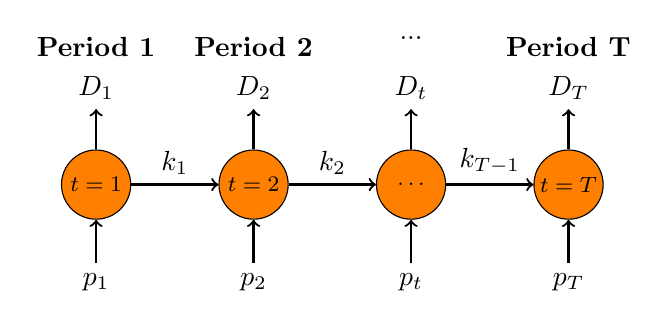
\begin{tikzpicture}[scale=1,
	node/.style={circle, fill=orange, draw, minimum size=2.5em, inner sep=1pt, font = \footnotesize}] 
		\node[below] at (0, 3) {\bf Period 1};                                                                                  
		\node[below] at (2, 3) {\bf Period 2};
		\node[below] at (4, 3) {...};
    	\node[below] at (6, 3) {\bf Period T};
    	\node[below] (11) at (0, 0) {$p_1$};                                                                                  
		\node[below] (21) at (2, 0) {$p_2$};
		\node[below] (31) at (4, 0) {$p_t$};
    	\node[below] (41) at (6, 0) {$p_T$};
    	\node[below] (12) at (0, 2.5) {$D_1$};                                                                                  
		\node[below] (22) at (2, 2.5) {$D_2$};
		\node[below] (32) at (4, 2.5) {$D_t$};
	    \node[below] (42) at (6, 2.5) {$D_T$};	    
		\node[node] (1) at (0, 1) {$t=1$};
		\node[node] (2) at (2, 1) {$t=2$};
		\node[node] (3) at (4, 1) {$\dots$};
		\node[node] (4) at (6, 1) {$t=T$};
		\draw[->, thick] (1) -- node[above] {$k_1$} (2);
		\draw[->, thick] (2) -- node[above] {$k_2$} (3) ;
		\draw[->, thick] (3) -- node[above] {$k_{T-1}$}(4);
		\draw[->, thick] (11) -- (1);
		\draw[->, thick] (21) -- (2);
		\draw[->, thick] (31) -- (3);
		\draw[->, thick] (41) -- (4);   
		\draw[->, thick] (1) -- (12);
		\draw[->, thick] (2) -- (22);
		\draw[->, thick] (3) -- (32);
		\draw[->, thick] (4) -- (42);                                     
	\end{tikzpicture}                    
	\caption{A schematic representation of the lot-sizing problem. Each node represents the material balance at each time period $t$.} \label{p1c1:fig:lot-sizing_diagram}		
\end{figure}

The production planning problem can be formulated as
%
\begin{flalign*}
	\mini & \sum_{t \in T} \left[C_t p_t + H s_t\right] \\
	\st 	  & p_t + k_{t-1} = D_t + k_t, ~\forall t \in T \\
	      & p_t, h_t \geq 0, ~\forall t \in T .	
\end{flalign*}
%

A few points must be considered carefully when dealing with lot-sizing problems. First, one must carefully consider boundary condition, that is, what the model is deciding in time periods $t = T$ and what is the initial inventory (carried from $t=0$). While the former will be seen by the model as the ``end of the world'', leading to the realization that optimal inventory levels at period $|T|$ must be zero, the latter might considerably influence how much production is needed during the planning horizon $T$. These must be observed and handled accordingly. 
 


\section{The geometry of LPs - graphical method} 

Let us now focus our attention to the geometry of linear programming (LP) models. As will become evident later on, LP models have a very peculiar geometry that is exploited by one of the most widespread methods to solve them, the \emph{simplex method}. 

\subsection{The graphical method}

In order to create a geometric intuition, we will utilise a graphical representation of the resource allocation example (the paint factory problem). But first, recall the general LP formulation \eqref{p1c1:eq:LP_objective}--\eqref{p1c1:eq:LP_domain}, where $A$ is an $m \times n$ matrix, and $b$, $c$, and $x$ have suitable dimensions. Let $a_i$ be one of the $m$ rows of $A$. Notice each constraint $a_i^\top x \leq b_i$ defines a closed half-space, with boundary defined by a hyperplane $a_i^\top x= b_i$, $\forall i \in I = \braces{1,\dots,m} \equiv [m]$ (we will return to these definitions in chapter 2; for now, just bear with me if these technical terms are unfamiliar to you). By plotting all of these closed half-spaces, we can see that their intersection will form the \emph{feasible region} of the problem, that is, the (polyhedral) set of points that satisfy all constraints $Ax \le b$. Figure \ref{p1c1:fig:feasible_region_plot} provides a graphical representation of the feasible region of the paint factory problem. 

\begin{figure}[h]
	\begin{subfigure}{0.45\textwidth}
		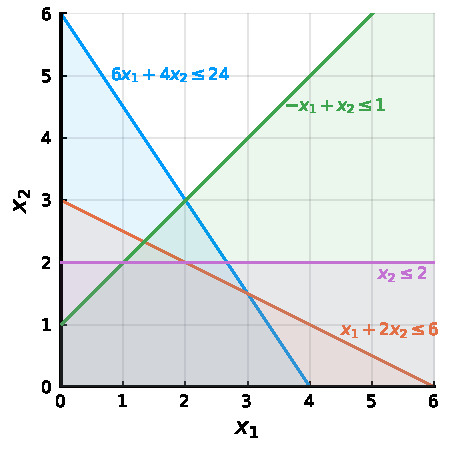
\includegraphics[scale=0.97]{part_1/chapter_1/figures/figure1-3a.pdf}	
		\caption{} \label{p1c1:fig:fig3a}
	\end{subfigure}
	\begin{subfigure}{0.45\textwidth}
		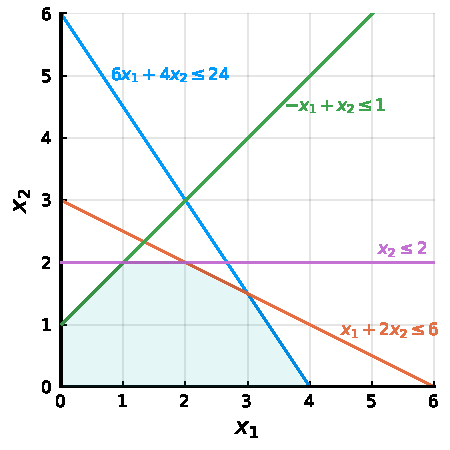
\includegraphics[scale=0.97]{part_1/chapter_1/figures/figure1-3b.pdf}
		\caption{} \label{p1c1:fig:fig3b}		
	\end{subfigure}
	\caption{The feasible region of the paint factory problem (in Figure \ref{p1c1:fig:fig3b}), represented as the intersection of the four closed-half spaces formed by each of the constraints (as shown in Figure \ref{p1c1:fig:fig3a}). Notice how the feasible region is a polyhedral set in $\reals^2$, as there are two decision variables ($x_1$ and $x_2$).} \label{p1c1:fig:feasible_region_plot}	
\end{figure}

We can use this visual representation to find the optimal solution for the problem, that is, the point $(x_1,x_2)$ within the feasible set such that the objective function value is maximal (recall that the paint factory problem is a maximisation problem). For that, we must consider how the objective function $z = c^\top x$ can be represented in the $(x_1, x_2)$-plane. Notice that the objective function forms a hyperplane in $(x_1, x_2, z) \subset \reals^3$, of which we can plot level curves (i.e., projections) onto the $(x_1, x_2)$-plane. Figure \ref{p1c1:fig:level_curves_a} shows the plotting of three level curves, for $z= 5, 10$, and $15$. 

This observation provides us with a simple graphical method to find the optimal solution to linear problems. One must simply sweep the feasible region in the direction of the gradient $\nabla z=[\frac{\partial z}{\partial x_1},\frac{\partial z}{\partial x_2}]^\top=[5,4]^\top$ (or in its opposite direction, if minimising) until one last point (or edge) of contact remains, meaning that the whole of the feasible region is behind that furthermost level curve. Figure \ref{p1c1:fig:level_curves_b} illustrates the process of finding the optimal solution for the paint factory problem.

\begin{figure}[h]
	\begin{subfigure}{0.45\textwidth}
		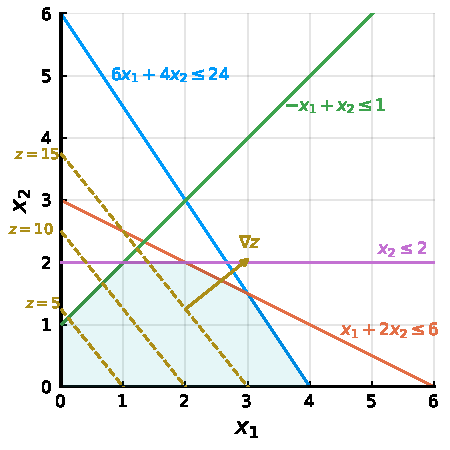
\includegraphics[scale=0.97]{part_1/chapter_1/figures/figure1-4a.pdf}  
		\caption{} \label{p1c1:fig:level_curves_a}	
	\end{subfigure}
	\begin{subfigure}{0.45\textwidth}
		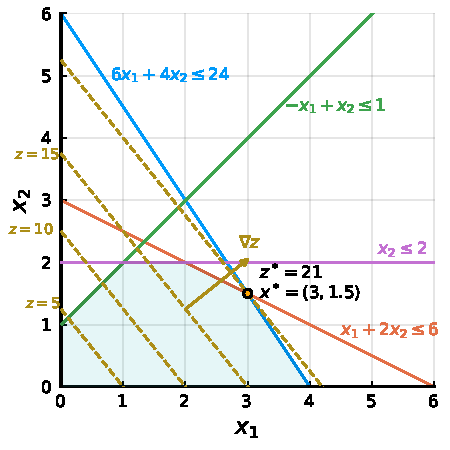
\includegraphics[scale=0.97]{part_1/chapter_1/figures/figure1-4b.pdf}
		\caption{} \label{p1c1:fig:level_curves_b}	 
	\end{subfigure}
	\caption{Graphical representation of some of the level curves of the objective function $z = 5x_1 + 4x_2$. Notice that the constant gradient vector $\nabla z = (5,4)^\top$ points to the direction in which the level curves increase in value. The optimal point is represented by $x^*=(3, 1.5)^\top$ with the furthermost level curve being that associated with the value $z^* = 21$}	
\end{figure}

The graphical method is important because it allows noticing several key features that will be used later on when we analyse a method that can search for optimal solutions for LP problems. The first is related to the notion of active or inactive constraints. We say that a constraint is \emph{active} at a given point $x$ if the constraint is satisfied as equality at the point $x$. For example, the constraints $6x_1 + 4x_2 \leq 24$ and $x_1 + 2x_2 \leq 6$ are active at the optimum $x^* = (3, 1.5)$, since $6(3) + 4(1.5) = 24$ and $3 + 2(1.5) = 6$. An active constraint indicates that the resource (or requirement) represented by that constraint is being fully depleted (or minimally satisfied). 

Analogously, \emph{inactive constraints} are constraints that are satisfied as strict inequalities at the optimum. For example, the constraint $-x_1 + x_2 \leq 1$ is inactive at the optimum, as $-(3) + 1.5 < 1$. In this case, an inactive constraint represents a resource (or requirement) that is not fully depleted (or is over-satisfied).


\subsection{Geometrical properties of LPs}

One striking feature concerning the geometry of LPs that becomes evident when we analyse the graphical method is that the number of candidate solutions is not infinite, but instead, only \emph{a finite set} of points are potential candidates for optimal solution. This is because the process of sweeping in the direction of the gradient of the (linear) objective function will, in general, lead to a unique solution that must lie on a vertex of the polyhedral feasible set. The only exceptions are either when the gradient $\nabla z$ happens to be perpendicular to a facet of the polyhedral set (and in the direction of the sweeping) or in case the sweeping direction is not bounded by some of the facets of the polyhedral set. These exceptional cases will be discussed in more detail later on, but, as we will see, the observation still holds.

In the graphical example (i.e., in $\reals^2$), notice how making $n = 2$ constraints active out of $m = 4$ constraints \emph{forms a vertex}. However, not all vertices are feasible. This allows us to devise a mechanism to describe vertices by activating $n$ of the $m$ constraints at a time, in which we could exhaustively test and select the best (i.e., that with the largest objective function value). The issue, however, is that the number of candidates increases \emph{exponentially} with the number of constraints and variables of the problem, which indicates this would quickly become computationally infeasible. As we will see, it turns out that this search idea can be made surprisingly efficient and is, in fact, the underlying framework of the \emph{simplex method}. However, there are indeed artificially engineered worst-case settings where the method does need to consider every single vertex.

The simplex method exploits the above idea to \emph{heuristically} search for solutions by selecting $n$ constraints to be active from the $m$ constraints available. Starting from an initial selection of constraints to be active, it selects one inactive constraint to activate and one to deactivate in a way that improvement in the objective function can be observed while feasibility is maintained. This process repeats until no improvement can be observed. In such a case, the \emph{geometry} of the problem guarantees \emph{(global) optimality}. In the following chapters, we will concentrate on defining algebraic objects that we will use to develop the simplex method.


\vfill
\pagebreak

\section{Exercises}

\subsection*{Exercise 1.1: Introduction to JuMP}
Use the Julia package JuMP.jl to implement the problems below and find the optimal solution. For the two-dimensional problems, use Plots.jl to illustrate the feasible region and the optimal solution.

\begin{enumerate}
	\item[(a)]
		\begin{flalign*}
			\maxi & x_1 + 2x_2 + 5x_3 &&\\
			\st   & x_1 - x_2 - 3x_3 \geq 5 &&\\
				  & x_1 + 3x_2 - 7x_3 \leq 10 &&\\
				  & x_1 \leq 10 &&\\
				  & x_1, x_2 \geq 0. &&
		\end{flalign*}

	\item[(b)]
		\begin{flalign*}
			\maxi & 2x_1 + 4x_2 &&\\
			\st   & x_1 + x_2 \leq 5 &&\\
			  	  & -x_1 + 3x_2 \leq 1 &&\\
	  			  & x_1 \leq 5 &&\\
				  & x_2 \leq 5 &&\\
				  & x_1, x_2 \geq 0. &&
		\end{flalign*}
	
	\item[(c)]
		\begin{flalign*}			
			\mini & -5x_1 + 10x_2 + x_3 + 2000x_4 &&\\
			\st   &  x_1 - x_2 \leq 1500 &&\\
				  & 4x_2 - x_3 \leq 5000x_4 &&\\
				  & x_1 + 3x_2 \geq 1000 &&\\
				  & x_1  \leq 10000 &&\\
				  & x_1, x_2 \in \reals, x_3 \leq 0, x_4 \in \braces{0,1}. &&
		\end{flalign*}

	\item[(d)]
		\begin{flalign*}	
			\maxi & 5x_1 + 3x_2 &&\\
			\st   & x_1 + 5x_2 \leq 3 &&\\
				  & 3x_1 - x_2 \leq 5 &&\\
				  & x_1 \leq 2 &&\\
 				  & x_2 \leq 30 &&\\
				  & x_1, x_2 \geq 0. &&
		\end{flalign*}
\end{enumerate}




\subsection*{Exercise 1.2: Transportation problem \cite{kwon2019julia}}
Consider the following network, where the supplies from the Austin and Buffalo nodes need to meet the demands in Chicago, Denver, and Erie. The data for the problem is presented in table below.

\begin{figure}[h]
	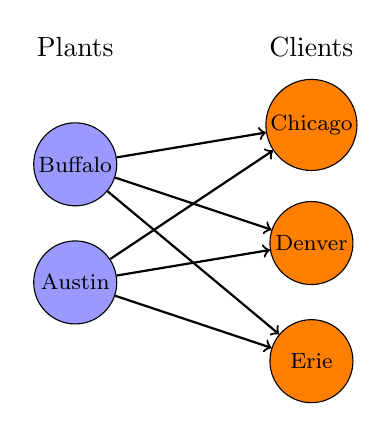
\begin{tikzpicture}[scale=1,
		node/.style={circle, fill=blue!40, draw, minimum size=3em, inner sep=1pt},
		node2/.style={circle, fill=orange, draw, minimum size=3em, inner sep=1pt}] 
    	\node[above] at (0, 4.75) {Plants};                                                                                  
    	\node[above] at (3, 4.75) {Clients};
	    \node[node] (1) at (0, 2) {\footnotesize Austin};
	    \node[node] (2) at (0, 3.5) {\footnotesize Buffalo};
	    \node[node2] (3) at (3, 4) {\footnotesize Chicago};
	    \node[node2] (4) at (3, 2.5) {\footnotesize Denver};
	    \node[node2] (5) at (3, 1) {\footnotesize Erie};
	    \foreach \x in {1,...,2} {
	       \foreach \y in {3,...,5} {
	          \draw[->, thick] (\x) -- (\y);
	          }}      
	\end{tikzpicture}
\end{figure}

\begin{table}[h]
	\begin{tabular}{r|ccc|c}
    	& & {\it Clients} &\\\hline
    	{\it Factory} & Chicago & Denver & Eire \\\hline
    	Buffalo 		  & 4       & 9      & 8    & 25 \\
    	Austin        & 10      & 7      & 9    & 600 \\\hline
    	Demands       & 15      & 12     & 13   & - \\\hline
	\end{tabular}
	\caption{Problem data: unit transportation costs, demands and capacities}
\end{table}

Solve the transportation problem, finding the minimum cost transportation plan.


\subsection*{Exercise 1.3: Capacitated transportation}
The Finnish company Next has a logistics problem in which used oils serve as raw material to form a class of renewable diesel. The supply chain team need to organise, to a minimal cost, the acquisition of two types of used oils (products p1 and p2) from three suppliers (supply nodes s1, s2, and s3) to feed the line of three of their used oils processing factories (demand nodes d1, d2, and d3). As the used oils are the byproduct of the supplier's core activities, the only requirement is that Next need to fetch the amount of oil and pay the transportation costs alone.

The oils have specific conditioning and handling requirements, so transportation costs vary between p1 and p2. Additionally, not all the routes (arcs) between suppliers and factories are available as some distances are not economically feasible. Table \ref{p1c1:tab:ex1-4_suplly_demand} shows the volume requirement of the two types of oil from each supply and demand node, and table \ref{p1c1:tab:ex1-4_arcs} show the transportation costs for each oil type per L and the arc capacity. Arcs with ``-'' for costs are not available as transportation routes.

\begin{table}[h!]
	\begin{subtable}[h]{0.4\textwidth}
		\begin{center}
		\begin{tabular}{c|cc}
			\textbf{node} & \textbf{p1} & \textbf{p2} \\
			\hline
			\textbf{s1 / d1} & 80 / 60 & 400 / 300 \\
			\textbf{s2 / d2} & 200 / 100 & 1500 / 1000 \\
			\textbf{s3 / d3} & 200 / 200 & 300 / 500 \\
		\end{tabular}
		\end{center}
		\caption{Supply availability and demand per oil type [in L]}
		\label{p1c1:tab:ex1-4_suplly_demand}
	\end{subtable}
	\hfill
	\begin{subtable}[h]{0.55\textwidth}
		\begin{center}
			\begin{tabular}{c|ccc}
				 & \textbf{d1} & \textbf{d2} & \textbf{d3}\\
				 & \textbf{p1/p2 (cap)} & \textbf{p1/p2 (cap)} & \textbf{p1/p2 (cap)}\\
				\hline
				\textbf{s1} & 5/- ($\infty$) & 5/18 (300) & -/- (0)\\
				\textbf{s2} & 8/15 (300) & 9/12 (700) & 7/14 (600)\\
				\textbf{s3} & -/- (0) & 10/20 ($\infty$) & 8/- ($\infty$)\\
			\end{tabular}
		\end{center}
		\caption{Arcs costs per oil type [in \euro \ per L] and arc capacities [in L]}
		\label{p1c1:tab:ex1-4_arcs}
	\end{subtable}
	\caption{Supply chain data}
\end{table}

Find the optimal oil acquisition plan for Next, i.e., solve its transportation problem to the minimum cost.


\subsection*{Exercise 1.4: The farmer's problem \cite{birge2011introduction}}
Consider a farmer who produces wheat, corn, and sugar beets on his 500 acres of land. During the winter, the farmer wants to decide 
how much land to devote to each crop. 

The farmer knows that at least 200 tons (T) of wheat and 240T of corn are needed for cattle feed. 
These amounts can be raised on the farm or bought from a wholesaler. Any production in excess of the feeding requirement would be sold. Over the last decade, mean selling prices have been \$ 170 and \$ 150 per ton of wheat and corn, respectively. The purchase prices are 40 \% more than this due to the wholesaler's margin and transportation costs.

Another profitable crop is sugar beet, which he expects to sell at \$36/T; however, the European Commission imposes a quota on sugar beet 
production. Any amount in excess of the quota can be sold only at \$10/T. The farmer’s quota for next year is 6000T.

Based on past experience, the farmer knows that the mean yield on his land is
roughly 2.5T, 3T, and 20T per acre for wheat, corn, and sugar beets, respectively.

Based on the data, build up a model to help the farmer allocate the farming area to each crop and how much to sell/buy of wheat, corn, 
and sugar beets considering the following cases.

\begin{itemize}
	\item[(a)] The predictions are 100\% accurate and the mean yields are the only realizations possible.	
	\item[(b)] There are three possible equiprobable scenarios (i.e, each one with a probability equal to $\frac{1}{3}$): a good, fair, and bad weather scenario. In the good weather, the yield is 20\% better than the yield expected whereas in the bad weather scenario it is reduced 20\% of the mean yield. In the regular weather scenario, the yield for each crop keeps the historical mean - 2.5T/acre, 3T/acre, and 20T/acre for wheat, corn, and sugar beets, respectively.
	\item[(c)]	What happens if we assume the same scenarios as item (b) but with probabilities 25\%, 25\%, and 50\% for good, fair, and bad weather, respectively? How the production plan changes and why?	
\end{itemize}


\vfill
\pagebreak
\subsection*{Exercise 1.5: Factory planning \cite{williams2013model}}
A factory makes seven products (PROD 1 to PROD 7) using the
following machines: four grinders, two vertical drills, three horizontal drills, one
borer and one planer. Each product yields a certain contribution to the profit (defined
as \$/unit selling price minus the cost of raw materials). These quantities (in \$/unit)
together with the unit production times (hours) required on each process are given
in Table \ref{p1c1:tab:ex1-5_prod_yield}. A dash indicates that a product does not require a process. 
There are also marketing demand limitations on each product each month. These are given in Table \ref{p1c1:tab:ex1-5_max_demand}.

\begin{table}[h]
	\begin{tabular}{l|lllllll}
		& \textbf{PROD1} & \textbf{PROD2} & \textbf{PROD3} & \textbf{PROD4} & \textbf{PROD5} & \textbf{PROD6} & \textbf{PROD7} \\ \hline 
		\textbf{Profit} & 10    & 6     & 8     & 4     & 11    & 9     & 3     \\
		\textbf{Grinding}              & 1.5   & 2.1   & –     & –     & 0.9   & 0.6   & 1.5   \\
		\textbf{Vert. drilling}     & 0.3   & 0.6   & –     & 0.9   & –     & 1.8   & –     \\
		\textbf{Horiz. drilling}   & 0.6   & –     & 2.4   & –     & –     & –     & 1.8   \\
		\textbf{Boring}                & 0.15  & 0.09  & –     & 0.21  & 0.3   & –     & 0.24  \\
		\textbf{Planing}               & –     & –     & 0.03  & –     & 0.15  & –     & 0.15 \\ \hline
	\end{tabular}
	\caption{Product yields}
	\label{p1c1:tab:ex1-5_prod_yield}
\end{table}

\begin{table}[H]
	\begin{tabular}{l|lllllll}
		& \textbf{PROD1} & \textbf{PROD2} & \textbf{PROD3} & \textbf{PROD4} & \textbf{PROD5} & \textbf{PROD6} & \textbf{PROD7} \\ \hline
		\textbf{January}   & 500   & 1000  & 300   & 300   & 800   & 200   & 100   \\
		\textbf{February}  & 600   & 500   & 200   & 0     & 400   & 300   & 150   \\
		\textbf{March}     & 300   & 600   & 0     & 0     & 500   & 400   & 100   \\
		\textbf{April}     & 200   & 300   & 400   & 500   & 200   & 0     & 100   \\
		\textbf{May}       & 0     & 100   & 500   & 100   & 1000  & 300   & 0     \\
		\textbf{June}      & 500   & 500   & 100   & 300   & 1100  & 500   & 60    \\ \hline
	\end{tabular}
	\caption{Maximum demand}
	\label{p1c1:tab:ex1-5_max_demand}
\end{table}

It is possible to store up to 100 of each product at a time at a cost of \$0.5 per unit per month. There are no stocks at present, but it is desired to have a stock of 50 of each type of product at the end of June. 

The factory works six days a week with two shifts of 8h each day. Assume that each month consists of only 24 working days. Also, there are no penalties for unmet demands. What is the factory's production plan (how much of which product to make and when) in order to maximise the total profit?






